\chapter{SLAM эксперименты}

Для проверки возможности использования SLAM методов совместно с методами построения и восстановления карты местности в реальном, было решено имитировать поток данный с БПЛА с помощью внешней usb веб-камеры.

\section{Настройка и калибровка камеры}

Для работы с usb веб-камерой через ROS, требуется использовать пакет \textbf{cv-camera} который предоставляет узел, взаимодействующий с камерой и принимающий от неё поток видео.

Как и во всех задачах компьютерного зрения, перед началом работы, требуется откалибровать камеру - то есть получить её внутренние и внешние параметры. С помощью калибровки получаются такие параметры, как: фокусное расстояние, угол наклона, и принципиальная точка (точка соответствующая центру фотографии) - которые образуют так называемую матрицу камеры и коэффициенты дисторсии (искажения).

\begin{figure}[h]
    \centering
    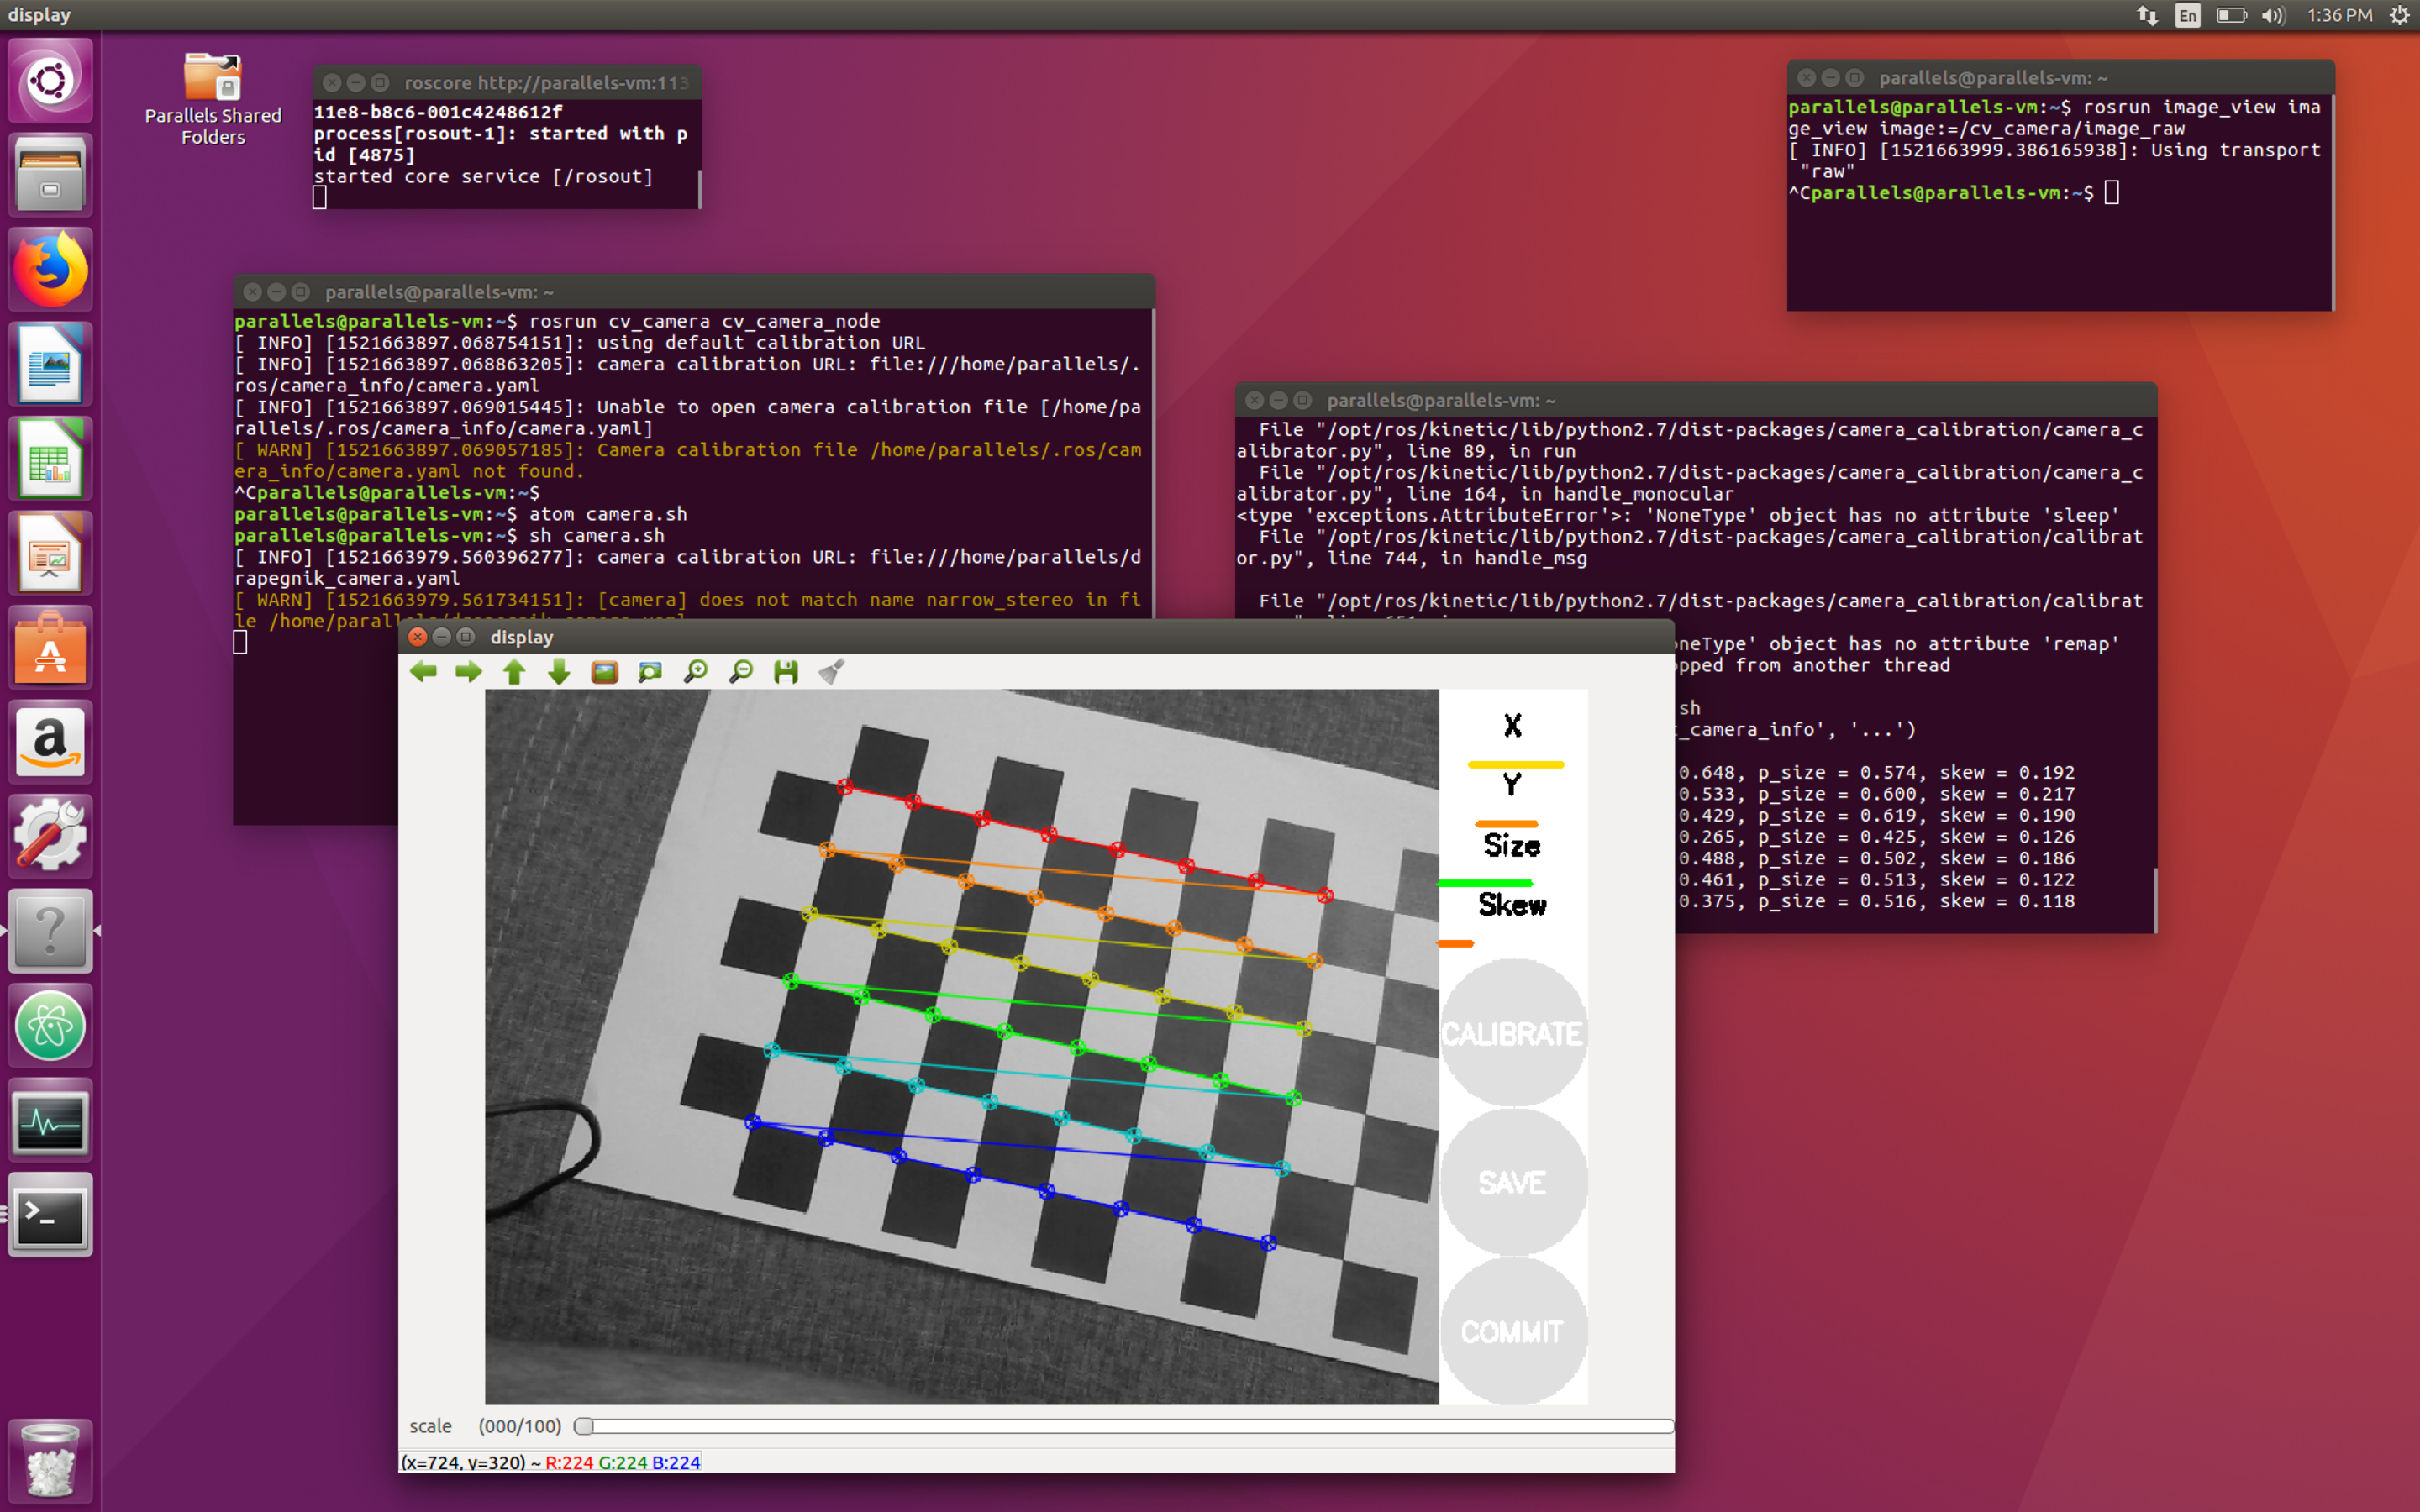
\includegraphics[width=0.9\textwidth]{images/chess.png}
    \caption{Калибровка камеры с помощью изображения шахматной доски}
    \label{fig:chess}
\end{figure}

Обычная процедура калибровки представляет из себя следующее:

\begin{enumerate}
    \item Выбор предмета с известной геометрией, обычно используется изображение шахматной доски;
    \item Подготовка 30 или более изображений выбранного предмета с разных ракурсов и расстояний;
    \item Определение ключевых точек на полученных фотографиях;
    \item Определение коэффициентов дисторсии через минимизацию ошибки.
    \item Нахождение остальных параметров через уравнения, полученные путем сопоставления изображений.
\end{enumerate}
 
Полученные параметры камеры экспортируются в файл и используются для конфигурации SLAM алгоритмов.

\section{Связывание через ROS}

\begin{figure}[h]
    \centering
    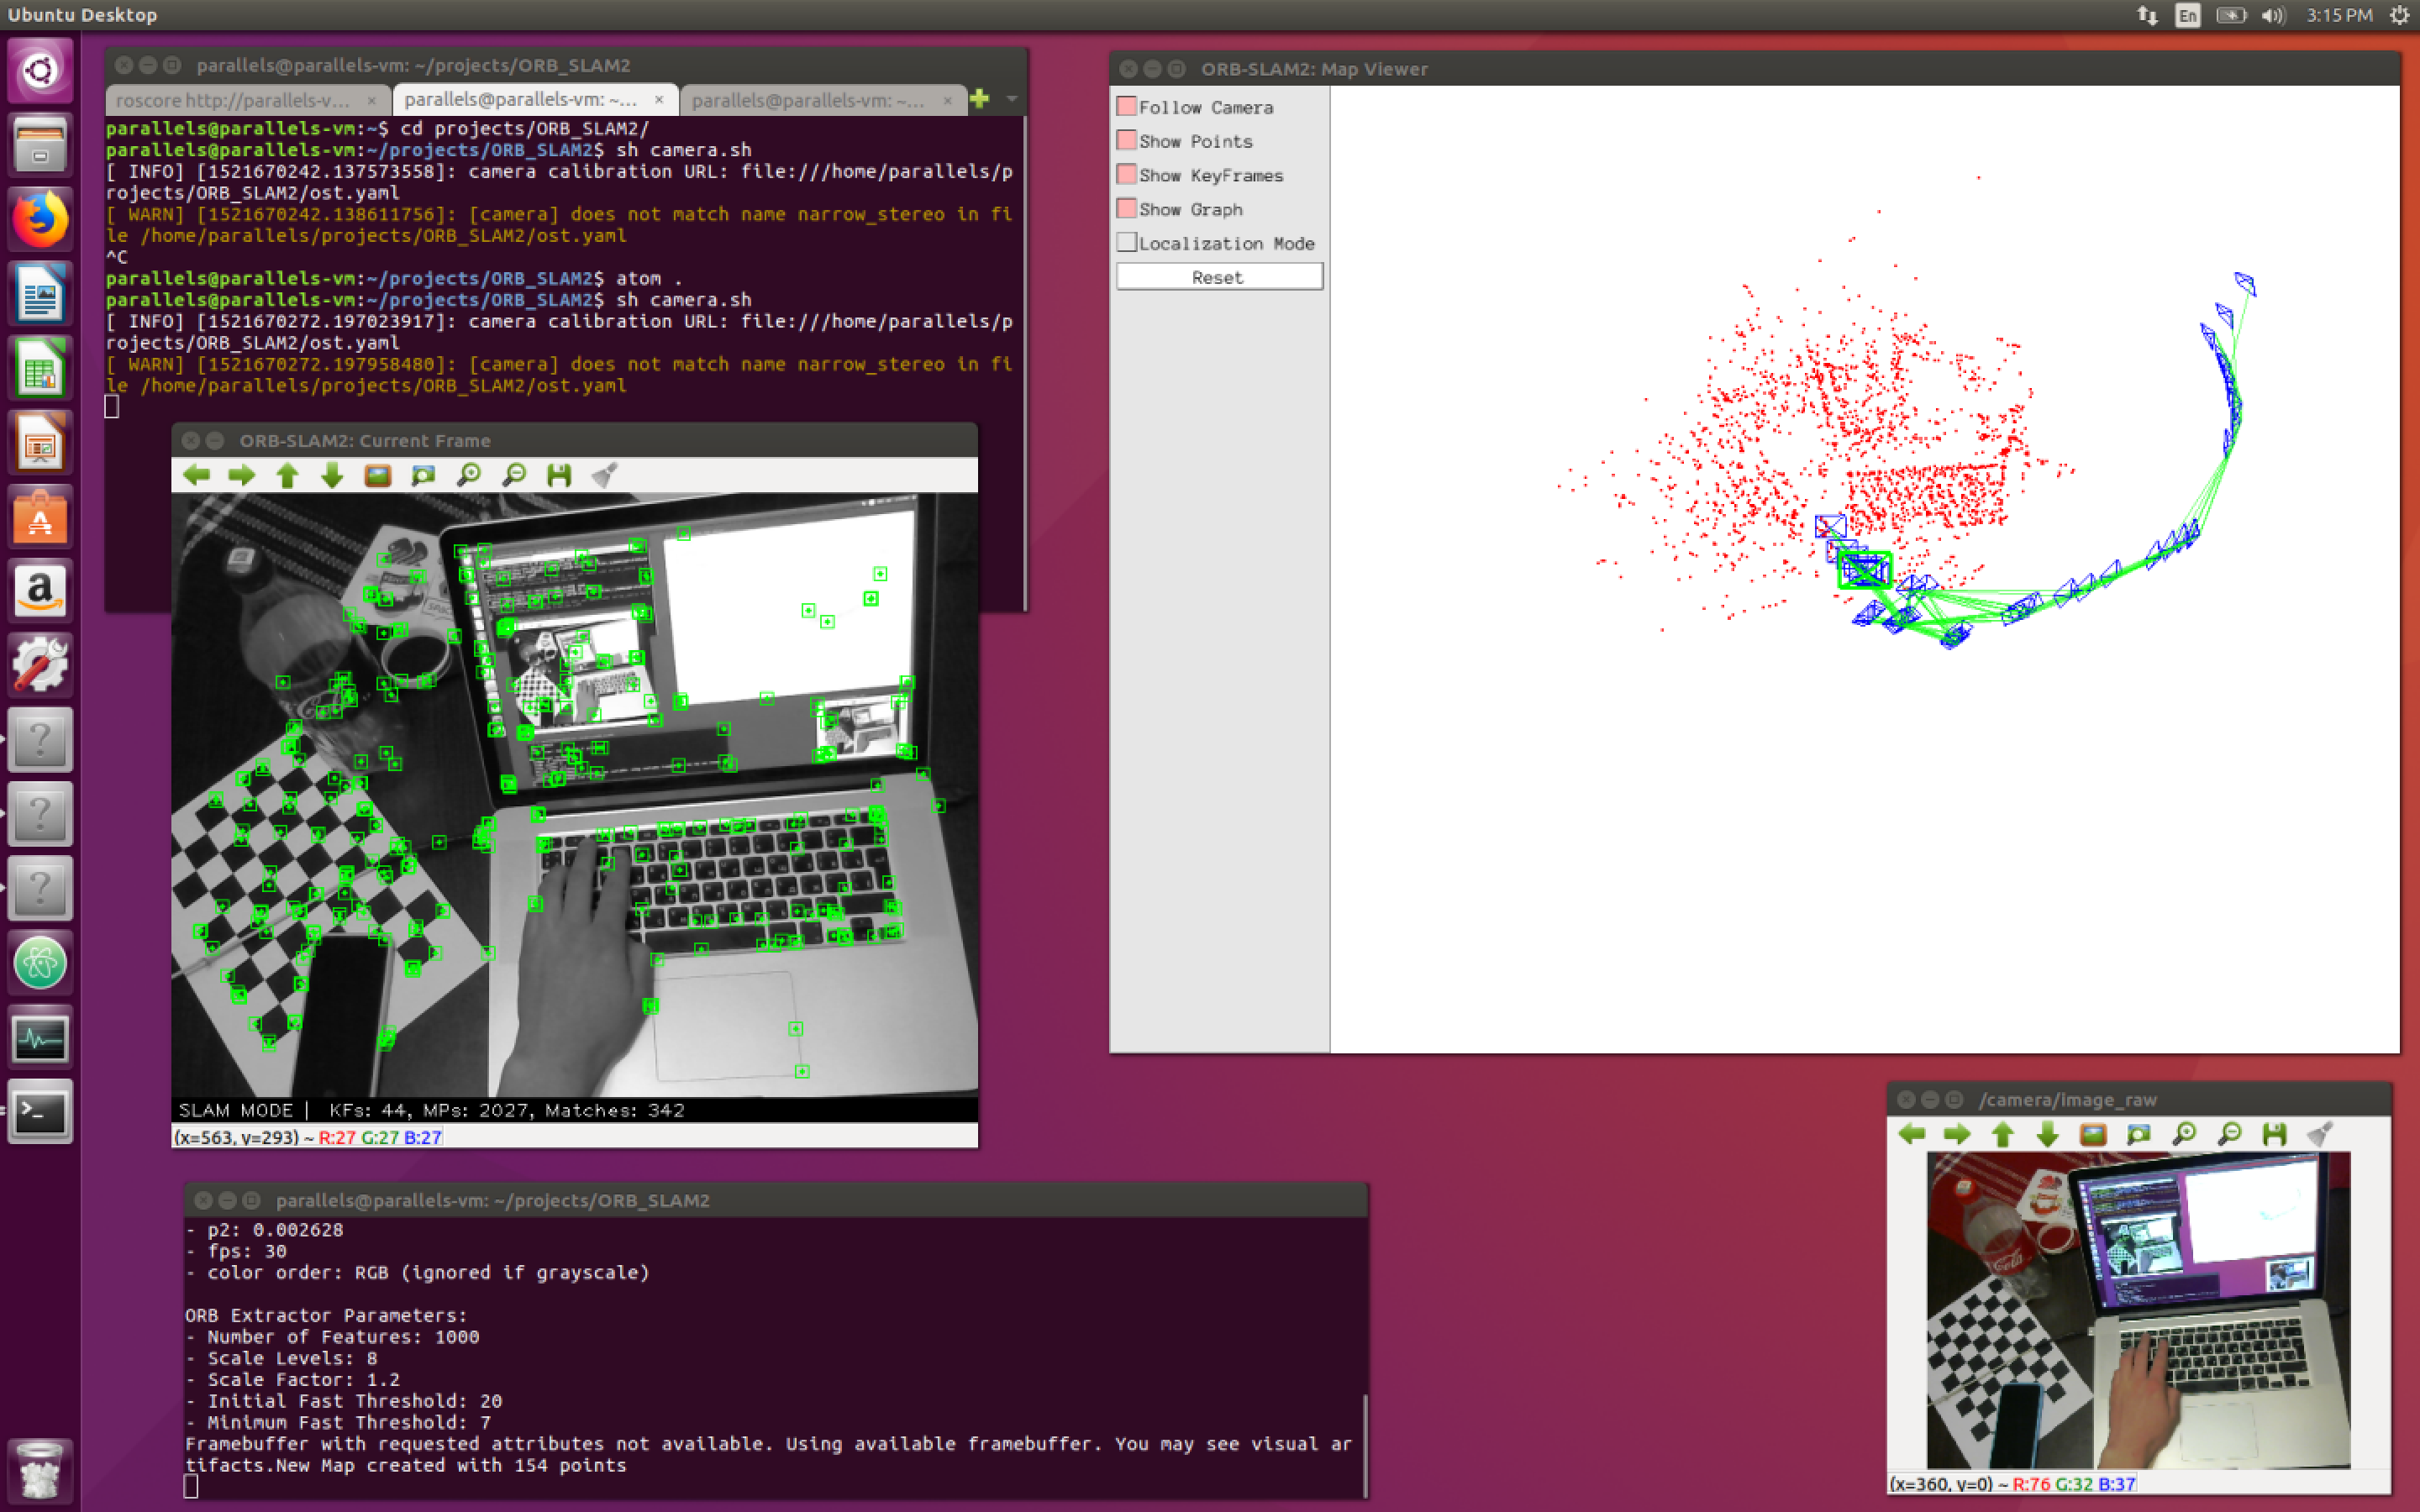
\includegraphics[width=1.0\textwidth]{images/ros-slam.png}
    \caption{Пример работы SLAM с веб-камерой}
    \label{fig:ros-slam}
\end{figure}

Для связывания и запуска всего вместе через ROS будем регистрировать и создавать новые узлы. Для начала создадим новый узел, который будет отвечать за веб-камеру. Он будет принимать от неё видео поток и публиковать его в специальный канал - \textbf{/cv\_camera/image\_raw}. Как альтернативу веб-камере можно использовать снимки из датасетов, которые упоминались ранее. Для этого напишем простой узел, в котором можно задать частоту кадров в секунду и директорию, в которой находятся снимки. Также можно указать имя канала в который узел будет публиковать снимки с заданной частотой. Последний вариант предпочтительнее для отладки и дебаге, так как не требует подключения веб-камеры и её перемещения в пространстве, что является утомительным процессом.

Далее SLAM запускается как отдельный узел и подписывается на канал с изображениями. При получении данных - отправляет их на процессы позиционирования и построения разряжённой карты точек. При определении положения камеры SLAM публикует эти данные в следующий канал. На этот канал, в свою очередь, подписано приложение и, при получении данных о камере, визуализирует её нанося на карту. После этого полученные от SLAM данные используются для инициализации процесса SFM, что ускоряет процесс построения плотной карты местности.